\documentclass{article}
\usepackage[utf8]{inputenc}

\title{13-05-20}
\author{giuseppe piombino}
\date{May 2021}

\usepackage{natbib}
\usepackage{graphicx}

\begin{document}

\maketitle

\section{Schnorr}
\subsection{Introduction}
In cryptography, a Schnorr signature is a digital signature produced by the Schnorr signature algorithm that was described by Claus Schnorr. It is a digital signature scheme known for its simplicity, among the first, whose security is based on the intractability of certain discrete logarithm problems. It is efficient and generates short signatures.
\subsection{Algorithm}
\subsubsection{Choosing parameters}
All users of the signature scheme agree on a group, G, of prime order, q, with generator,  g, in which the discrete log problem is assumed to be hard. Typically a Schnorr group is used.
All users agree on a cryptographic hash function $H:\{0,1\}^{*} \rightarrow {{Z}}_{q}$. 
A group is a set equipped with a binary operation that combines any two elements to form a third element in such a way that associativity, identity (neutral element) and invertibility (possibility to negate or have a reciprocal quantity) are satisfied.
A Schnorr group, proposed by Claus P. Schnorr, is a large prime-order subgroup of ${  {Z} _{p}^{\times }}$, the multiplicative group of integers modulo ${ p}$ for some prime  p. To generate such a group, generate p, q, r such that ${ p=qr+1}$ with ${ p} , { q}$  prime. Then choose any ${ h}$  in the range ${ 1<h<p}$  until you find one such that
${ h^{r}\not \equiv 1\;({{mod}}\;p)} $.
This value
${ g=h^{r}{{ mod }}p}$ 
is a generator of a subgroup of ${ {Z} _{p}^{\times }}$  of order ${ q}$.
P, is chosen to be large enough to resist index calculus and related methods of solving the discrete-log problem (perhaps 1024 to 3072 bits), while   is large enough to resist the birthday attack on discrete log problems, which works in any group (perhaps 160 to 256 bits). Because the Schnorr group is of prime order, it has no non-trivial proper subgroups, thwarting confinement attacks due to small subgroups. Implementations of protocols that use Schnorr groups must verify where appropriate that integers supplied by other parties are in fact members of the Schnorr group; ${ x}$ is a member of the group if ${ 0<x<p}$ and ${ x^{q}\equiv 1\;({{mod }}p)}$. Any member of the group except the element   is also a generator of the group.
\subsubsection{Notation}
In the following,
\begin{itemize}
    \item Exponentiation stands for repeated application of the group operation
    \item Juxtaposition stands for multiplication on the set of congruence classes or application of the group operation (as applicable)
    \item Subtraction stands for subtraction on the set of congruence classes ${ M\in \{0,1\}^{*}}$, the set of finite bit strings
    \item $s,e,e_{v} c {Z} _{q}$, the set of congruence classes modulo ${ q}$ (with congruence classes we mean the group of number whose modulo q is the same)
    \item ${ x,k\in {Z} _{q}^{\times}}$, the multiplicative group of integers modulo q (for prime  q,  ${Z}_{q}^{\times}={Z}_{q} \setminus {\overline {0}}_{q}$ ) (they can be seen as a set of congruence of modulo q that are also coprime of q. a coprime couple of number are 2 integer that share as dividend only 1)
    \item ${ y,r,r_{v}\in G}$ .

\end{itemize}
\subsubsection{Key generation}
Choose a private signing key, ${ x}$ , from the allowed set.
The public verification key is ${ y=g^{x}}$.
\subsubsection{Signing}
To sign a message, ${ M}$:

Choose a random ${ k}$ from the allowed set.
\begin{itemize}
    \item Let ${ r=g^{k}}r=g^{k}$.
    \item Let ${ e=H(r\parallel M)}$, where ${ \parallel }$  denotes concatenation and ${ r}$ is represented as a bit string.
    \item ${ s=k-xe}$.
\end{itemize}
The signature is the pair, ${ (s,e)}$.

Note that ${ s,e\in {Z} _{q}}$; if ${ q<2^{160}}$, then the signature representation can fit into 40 bytes.


\subsubsection{Verifying}
\begin{itemize}
    \item Let ${ r_{v}=g^{s}y^{e}}$
    \item Let ${ e_{v}=H(r_{v}\parallel M)}$

\end{itemize}
If ${ e_{v}=e}$ then the signature is verified.

\subsubsection{Proof of correctness}
It is relatively easy to see that ${ e_{v}=e}$ if the signed message equals the verified message:

${ r_{v}= g^{s}y^{e}= g^{k-xe}g^{xe}= g^{k}=r}$, and hence ${ e_{v}=H(r_{v}\parallel M)=H(r\parallel M)=e}$.

Public elements: ${ G}$, ${ g}$, ${ q}$, ${ y}$, ${ s}$, ${ e}$, ${ r}$. Private elements: ${ k}$, ${ x}$.

This shows only that a correctly signed message will verify correctly; many other properties are required for a secure signature algorithm.

\subsubsection{Key leakage from nonce reuse}
Just as with the closely related signature algorithms DSA, ECDSA, and ElGamal, reusing the secret nonce value ${ k}$ on two Schnorr signatures of different messages will allow observers to recover the private key. In the case of Schnorr signatures, this simply requires subtracting ${ s}$ values:
${ s'-s=(k'-k)-x(e'-e)}$.
If ${ k'=k}$ but ${ e'\neq e}$ then ${ x}$ can be simply isolated. In fact, even slight biases in the value ${ k}$ or partial leakage of ${ k}$ can reveal the private key, after collecting sufficiently many signatures and solving the hidden number problem.

\subsubsection{Short Schnorr signatures}
The aforementioned process achieves a t-bit security level with 4t-bit signatures. For example, a 128-bit security level would require 512-bit (64-byte) signatures. The security is limited by discrete logarithm attacks on the group, which have a complexity of the square-root of the group size.

In Schnorr's original 1991 paper, it was suggested that since collision resistance in the hash is not required, then therefore shorter hash functions may be just as secure, and indeed recent developments suggest that a t-bit security level can be achieved with 3t-bit signatures. Then, a 128-bit security level would require only 384-bit (48-byte) signatures, and this could be achieved by truncating the size of e until it is half the length of the s bitfield.

\subsubsection{Bitcoin}

Bitcoin currently uses the ECDSA algorithm to generate cryptographic signatures for a given message and secp256k1 keypair. Schnorr is an alternative algorithm with several advantages. One key advantage is that when multiple keys are used to sign the same message with Schnorr, the resulting signatures can be combined into a single signature. This can be used to significantly reduce the size of multisig (multi-signature) payments and other multisig related transactions, for example lightning channel transactions.
The main reason that Bitcoin did not originally use Schnorr signatures is that Schnorr was not standardized, and was not available in common crypto libraries.
Schnorr signatures are a proposed future extension that give a new way to generate signatures (R,s) on a hash h.
An advantage of this method is that, if parties cooperate, we can generate a single signature that validates two or more separate transactions.
Given a hash value h, hash function f(), private key x, group generator G, and public key P=xG, we can generate a Schnorr signature on h as follows (here 1 and 2 are the two side of the communication):
Choose h1, h2, x1, x2, G, P1=Gx1, P2=Gx2. Each party chooses a nonce yielding k1 and k2, and publicly shares R1=Gk1, R2=Gk2.
Let R = R1+R2. Each signer generates an s, $s1 = k1 - f(h \parallel R \parallel P)x1$, $s2 = k2 - f(h \parallel R \parallel P)x2$. The signature (R, s) where s = s1 + s2 proves both transactions are signed.
Note that \[sG = (s1 + s2)G = s1G + s2G \]
\[=(k1 - f(h \parallel R \parallel P)x1)G + (k2 - f(h \parallel R \parallel P)x2)G \]
\[=k1G - f(h \parallel R \parallel P)x1G + k2G - f(h \parallel R \parallel P)x2G \]
\[=R1 + R2 - f(h \parallel R \parallel P)(P1 + P2) = R - f(h \parallel R \parallel P)(P1 + P2)\]
To verify, check that $sG +f(h \parallel R \parallel P)(P1+P2)$ is R.
This can be easily generalized from 2 to N.
\section{Subliminal channel}
\subsection{Introduction}
Covert channels transport information by using a system parameter that was not intentionally made for communication. System parameters can be, e.g., jitter, crosstalk, modulation, key material, padding, nonce or random values. Subliminal channels are a subgroup of covert channels. They are hard to detect and can be used to communicate secretly over an insecure channel with help of digital signatures
In [Sim84] Gustavus J. Simmons presented how the “Prisoner Problem” can be solved with help of digital signature crypto systems. The prisoner problem describes the problem how two prisoners can communicate confidentially and undetected over an insecure channel, the warden. Remaining undetected is the main problem here because the warden must read all communication.
\subsection{Prisoner problem}
The prisoners agree on the following scheme before they are arrested, such that the warden has no knowledge about this agreement. The setting is that two prisoners want to communicate and the only way is the warden. The prisoners cannot use encryption because the warden wants to read all communication or he will not deliver the message. They decide to sign the outcome of a fair-coin toss and use the signature of the authentication system to hide their communication.
For simplicity a three bit message is used and the warden only accepts an even parity message when head is the outcome of the coin toss and at tail an odd parity message. The eight (23 = 8) possible messages are now sorted into two unique sets. Both sets contain two even and two odd parity messages, e.g., $\phi = {000, 101, 010, 111}$ and $\psi = {110, 011, 100, 001}$.
If the set $\phi$ is associated with “1” and $\psi$ with “0” the prisoners can communicate a 1-bit subliminal message independently from the outcome of the toss and the warden cannot detect this message.
\subsection{DSA example}
The Digital Signature Algorithm has one subliminal broadband[3] and three subliminal narrow-band channels [4]

At signing the parameter ${ k}$ has to be set random. For the broadband channel this parameter is instead set with a subliminal message ${ m'}$.
\begin{enumerate}



\item Key generation
\begin{enumerate}
    \item choose prime ${ p=2347}$
    \item choose prime ${ q=23}$
    \item calculate generator ${ g=266}$
    \item choose authentication key ${ x=1468}$ and send it securely to the receiver
    \item calculate public key ${ y=g^{x}}$ mod ${ p=2100}$
\end{enumerate}
\item Signing
\begin{enumerate}
    \item choose message ${ m=1337}$ (hash function ${ H(m)}$ is here substituted with a modulo reduction by 107) calculate message hash value ${ h=m}$ mod ${ q=1337}$ mod ${ 107=53}$
    \item instead of random value ${ k=?}$ subliminal message ${ m'=17}$ is chosen
    \item calculate inverse of the subliminal message ${ m'^{-1}=19}$ mod ${ 23}$
    \item calculate signature value ${ r=(g^{k}}$ mod \  ${ p)}$ mod \ ${ q=(266^{17}}$ mod \ ${ 2347)}$ mod \ ${ 23=12}$
    \item calculate signature value \[{ s=k^{-1}*(h+x*r)} \ mod \ { q=19*(53+1468*12)}\  mod\  { 23=3}\]
    \item sending message with signature triple ${ (1337;12,3)}$
\end{enumerate}
\item Verifying
\begin{enumerate}
    \item receiver gets message triple ${ (m;r,s)=(1337;12,3)}$
    \item calculate message hash ${ h=H(m)}$ mod ${ q=1337}$ mod ${ 107=53}$
    \item calculate inverse ${ w=s^{-1}}$ mod ${ q=8}$
    \item calculate ${ u_{1}=(h*w)}$ mod ${ q=53*8}$ mod { 23=10}23 = 10
    \item calculate ${ u_{2}=(r*w)}$ mod ${ q=12*8}$ mod ${ 23=4}$
    \item calculate signature ${ v=(g^{u_{1}}*y^{u_{2}}}$ mod ${ p)}$ mod ${ q=(266^{10}*2100^{4}}$ mod ${ 2347)}$ mod ${ 23=12}$
    \item since ${ v=r}$, the signature is valid
\end{enumerate}
\item Message extraction on receiver side
\begin{enumerate}
    \item from triple (1337; 12, 3)
    \item extract message ${ m'=8*(53+1468*12)}$ mod ${ 23=17}$
\end{enumerate}
\end{enumerate}
The formula for message extraction is derived by transposing the signature value ${ s}$ calculation formula.
\begin{itemize}
    \item ${ s=m'^{-1}*(h+xr)}$ mod ${ q}$
    \item ${ s*m'=h+xr}$ mod ${ q}$
    \item ${ m'=s^{-1}*(h+xr)}$ mod ${ q}$
\end{itemize}
\subsection{Narrowband}
The system described is a broadband channel. Another way of communicate is to use just part of the channel avoiding to share the authentication key. Simmons describes three narrowband channels in [Sim93]. For the first narrowband channel sender and receiver have to create a shared secret prime P with P > q. The public prime p should not be used, because anybody can check the following explanations with p and therefore would be able to disclose the usage of the subliminal channel. One bit can be transmitted subliminally if the parameter r is or is not a quadratic residue modulo P.
For the first narrowband channel assume the transmitter and the receiver has securely exchanged the prime $P = 2237$. For the broadband channel example value $r = 12$ we calculate $r^{(P-1)/2} mod \ P = 12^{1118} mod \ 2237 = -1$. This is a quadratic non-residue and if we would associate quadratic residues with the value 1 we would have transmitted a 0 in our broadband example. For$ k = 15$ we get $r = (g^{k} \ mod \ p) \ mod \ q = (266^{15} \ mod \ 2347)\  mod \ 23 = 11$. If we check $r^{(P-1)/2} \ mod \ P = 11^{1118} mod \ 2237 = 1$ and therefore this is a quadratic residue.
More about narrow band and subliminal channel is at this link:

\[https://www.emsec.ruhr-uni-bochum.de/media/crypto/\]
\[attachments/files/2011/03/subliminal_channels.pdf\]
\section{Blinding signature}
\subsection{Introduction}
In cryptography, blinding is a technique by which an agent can provide a service to (i.e., compute a function for) a client in an encoded form without knowing either the real input or the real output. Blinding techniques also have applications to preventing side-channel attacks on encryption devices.
More precisely, Alice has an input x and Oscar has a function f. Alice would like Oscar to compute y = f(x) for her without revealing either x or y to him. The reason for her wanting this might be that she doesn't know the function f or that she does not have the resources to compute it. Alice "blinds" the message by encoding it into some other input E(x); the encoding E must be a bijection on the input space of f, ideally a random permutation. Oscar gives her f(E(x)), to which she applies a decoding D to obtain D(f(E(x))) = y.
Blind signatures can also be used to provide unlinkability, which prevents the signer from linking the blinded message it signs to a later un-blinded version that it may be called upon to verify. In this case, the signer's response is first "un-blinded" prior to verification in such a way that the signature remains valid for the un-blinded message. This can be useful in schemes where anonymity is required.
\begin{figure}[h!]
\centering
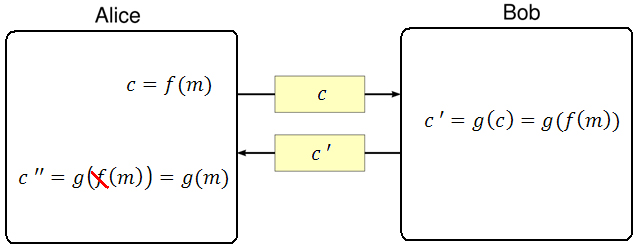
\includegraphics[scale=0.5]{BlindSignature.jpg}
\end{figure}
\subsection{Carbon envelope parallelism}
An often-used analogy to the cryptographic blind signature is the physical act of a voter enclosing a completed anonymous ballot in a special carbon paper lined envelope that has the voter's credentials pre-printed on the outside. An official verifies the credentials and signs the envelope, thereby transferring their signature to the ballot inside via the carbon paper. Once signed, the package is given back to the voter, who transfers the now signed ballot to a new unmarked normal envelope. Thus, the signer does not view the message content, but a third party can later verify the signature and know that the signature is valid within the limitations of the underlying signature scheme.
\begin{figure}[h!]
\centering
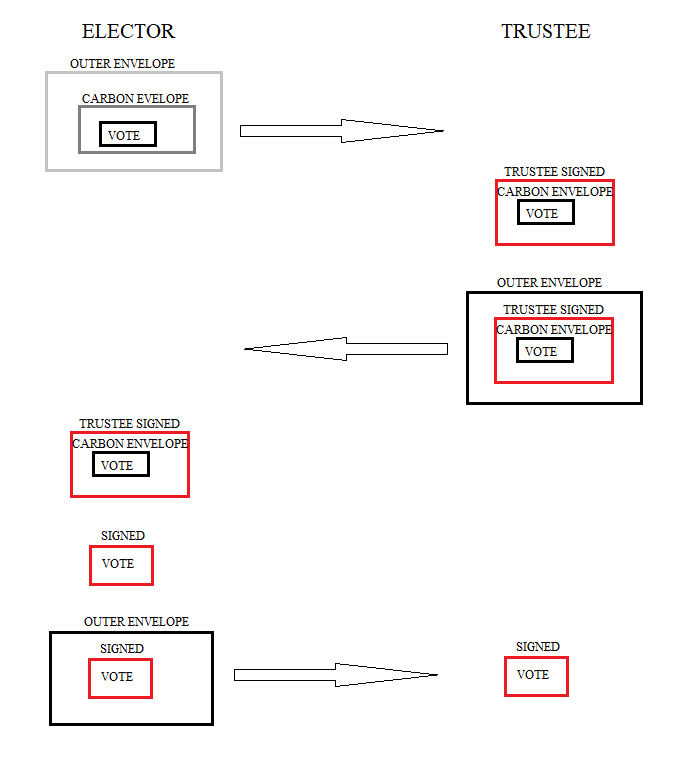
\includegraphics[scale=0.7]{BlindedSignature.png}
\end{figure}
\subsection{Application}
Its main application is the banking sector, as well as the scope of e-voting. As is known, the automation of the payment process has been going on for a long time. At the same time, with the use of electronic payment systems, the bank always has full information about who, where, when and to whom the funds transferred. This fact has a significant impact on the privacy of users. Using a blind e-signature allows the creation of such payment systems, which are able to ensure the anonymity of payments, but at the same time, give users the ability, if necessary, to prove the fact of payment, for example in the case of litigation, and the ability to stop use of payments media reported  stolen.
\subsection{Blind RSA signatures}
One of the simplest blind signature schemes is based on RSA signing. A traditional RSA signature is computed by raising the message m to the secret exponent d modulo the public modulus N. The blind version uses a random value r, such that r is relatively prime to N (i.e. gcd(r, N) = 1). r is raised to the public exponent e modulo N, and the resulting value ${ r^{e} {mod\, {N}}}$ is used as a blinding factor. The author of the message computes the product of the message and blinding factor, i.e.:

${ m'\equiv mr^{e}\ (\mathrm {mod} \, N)}$
and sends the resulting value ${ m'}$ to the signing authority. Because r is a random value and the mapping ${ r\mapsto r^{e}{ mod\, {N}}}$ is a permutation it follows that ${ r^{e}{ mod\, {N}}}$ is random too. This implies that ${ m'}$ does not leak any information about m. The signing authority then calculates the blinded signature s' as:

${ s'\equiv (m')^{d}\ (\mathrm {mod} \ N).}$
s' is sent back to the author of the message, who can then remove the blinding factor to reveal s, the valid RSA signature of m:

${ s\equiv s'\cdot r^{-1}\ (\mathrm {mod} \ N)}$
This works because RSA keys satisfy the equation ${ r^{ed}\equiv r{\pmod {N}}}$ and thus

${ s\equiv s'\cdot r^{-1}\equiv (m')^{d}r^{-1}\equiv m^{d}r^{ed}r^{-1}\equiv m^{d}rr^{-1}\equiv m^{d}{\pmod {N}},}$
hence s is indeed the signature of m.

In practice, the property that signing one blinded message produces at most one valid signed messages is usually desired. This means one vote per signed ballot in elections, for example. This property does not hold for the simple scheme described above: the original message and the unblinded signature is valid, but so is the blinded message and the blind signature, and possibly other combinations given a clever attacker. A solution to this is to blind sign a cryptographic hash of the message, not the message itself.

\subsection{Dangers of RSA blind signing}
RSA is subject to the RSA blinding attack through which it is possible to be tricked into decrypting a message by blind signing another message. Since the signing process is equivalent to decrypting with the signer's secret key, an attacker can provide a blinded version of a message ${ m}$ encrypted with the signer's public key, ${ m'}$ for them to sign. The encrypted message would usually be some secret information which the attacker observed being sent encrypted under the signer's public key which the attacker wants to learn more about. When the attacker removes the blindness the signed version they will have the clear text:

$ m''m'r^{e}{mod\, {n}}= $
$(m^{e}{ mod\, {n}}\cdot r^{e}){ mod\, {n}}=$
$(mr)^{e}{ mod\, {n}}$
where ${ m'}$ is the encrypted version of the message. When the message is signed, the cleartext ${ m}$ is easily extracted:

\[ s'=m''^{d}{ mod\, {n}} \] 
\[=((mr)^{e}{ mod\, {n}})^{d}{ mod\, {n}}\]
\[=(mr)^{ed}{mod\, {n}}\]
\[=m r{ mod {n}}{\mbox{, since }}ed\equiv 1 {mod {\phi (n)}}\]
Note that ${ \phi (n)}$ refers to Euler's totient function. The message is now easily obtained.

${ m=s' r^{-1}{ mod {n}}}$
This attack works because in this blind signature scheme the signer signs the message directly. By contrast, in an unblinded signature scheme the signer would typically use a padding scheme (e.g. by instead signing the result of a cryptographic hash function applied to the message, instead of signing the message itself), however since the signer does not know the actual message, any padding scheme would produce an incorrect value when unblinded. Due to this multiplicative property of RSA, the same key should never be used for both encryption and signing purposes.



\end{document}